
\chapter{Introduction}

\section{Sources of Similarities}

Note that functions that are identical at the IR or machine level are not
necessarily identical at the source level.
Figure~\ref{fig:identical-example} shows two real functions extract from the
447.dealII program in the SPEC CPU2006~\cite{spec} benchmark suite.
Although these two functions are not identical at the source level, they become
identical after a template specialization and some optimizations are applied, in
particular, constant propagation, constant folding, and dead-code elimination. 
Specializing \verb|dim| to $1$ enables to completely remove the loop in the
function \verb|PolynomialSpace|.
Similarly, specializing \verb|dim| to $1$ results in only the first iteration
of the loop in the function \verb|TensorProductPolynomials| being executed.
The compiler is able to statically analyze and simiplify the loops in both
functions, resulting in the identical functions shown at the bottom of
Figure~\ref{fig:identical-example}.

\begin{figure}[h]
\centering
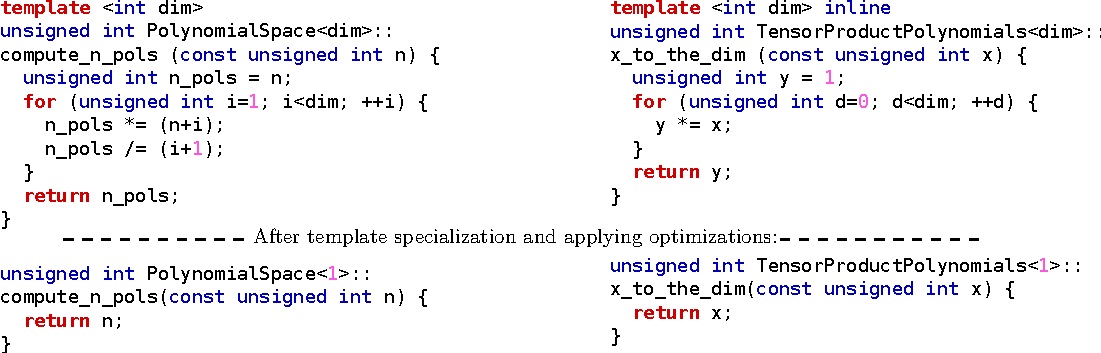
\includegraphics[width=\textwidth]{src/intro/figs/identical-example}
\caption{Two function extracted from the 447.dealII benchmark that are not
           identical at the source level, but after applying template
           specialization and optimizations they become identical at the IR
           level.}
\label{fig:identical-example}
\end{figure}


Identical code is particularly common in C++ programs
with heavy use of \textit{parametric polymorphism}, via template or \textit{auto} type deduction.
